
% This LaTeX was auto-generated from an M-file by MATLAB.
% To make changes, update the M-file and republish this document.

\documentclass{article}
\usepackage{graphicx}
\usepackage{color}

\sloppy
\definecolor{lightgray}{gray}{0.5}
\setlength{\parindent}{0pt}

\begin{document}

    
    
\section*{}


\subsection*{Contents}

\begin{itemize}
\setlength{\itemsep}{-1ex}
   \item CSC8580 Network Performance \& Management -
   \item Initialization
   \item Part 1a - load data
   \item Part 1b - Initialize Storage For Aggregates
   \item Part 2 - Perform Aggregate Bitrate
   \item Part 3 - Plot Data By Hour
   \item Part 4 - Provider Analysis
\end{itemize}


\subsection*{CSC8580 Network Performance \& Management -}

\begin{verbatim}
%{
  Suleyman Muhammad
  Graduate Computer Engineer
  Villanova University Class '10
  Villanova Grad Class '11
  Final Project 2011 CSC8580: Network Management and Performance
%}
\end{verbatim}


\subsection*{Initialization}

\begin{verbatim}
clc;clear;close all

Submitted=datestr(now, 21)

cd('W:\Multimedia_GRAD\matlabCSC8580')
\end{verbatim}

        \color{lightgray} \begin{verbatim}
Submitted =

Apr.27,2011 14:11:25

\end{verbatim} \color{black}
    

\subsection*{Part 1a - load data}

\begin{verbatim}
dat = csvread('cdat2.csv'); %Load in CVS file
[m n] = size(dat);
\end{verbatim}


\subsection*{Part 1b - Initialize Storage For Aggregates}

\begin{verbatim}
%Clear Unused Variables for use with aggregate
dat(:,5) = zeros(m,1);
\end{verbatim}


\subsection*{Part 2 - Perform Aggregate Bitrate}

\begin{verbatim}
for i = 1:m
   start   = dat(i,1); % Start time
   vsecs   = dat(i,2); % Vewing seconds
   bitrate = dat(i,3); % Bitrate
   for j = 1:(vsecs-1) % From the start time, for each veiwing sec
                       % increment the corresponding slot by the bitrate
       k=j-dat(1,1);
       %%AGGREGATE BITRATE
       dat((dat(i,1)+k),5) = dat(dat(i,1)+k,5) + dat(i,3);
   end
end

% Clear loop variables
clear i j k start vsecs bitrate;
\end{verbatim}


\subsection*{Part 3 - Plot Data By Hour}

\begin{verbatim}
half    = 30*60;     % Half hour in seconds
hour_s  = 60*60;     % One hour in seconds
day_s   = hour_s*24; % One day in seconds

day1=dat(1:day_s,5);         % Oct. 18th aggregate
day2=dat(day_s+1:2*day_s,5); % Oct. 19th aggregate
dayAVE = (day1+day2)/2;      % Average of 10/18/10 and 10/19/10

% Plot day 1 aggregate
figure (1)
plot(day1)
title('Bit Rate vs Time: 12am-11pm October 18th 2010')
 xlabel('Time (Hrs)')
 ylabel('Bit Rate')
 set(gca, 'XTick', 1:hour_s:day_s)
 set(gca, 'XTickLabel',{'12am','','','3am','','','6am','','','9am','',...
                        '','12pm','','','3pm','','', '6pm', '', '',...
                        '9pm','','11pm'})

% Plot day 2 aggregate
figure (2)
plot(day2)
title('Bitrate vs Time: 12am-11pm October 19th 2010')
 xlabel('Time (Hrs)')
 ylabel('Bit Rate')
 set(gca, 'XTick', 1:hour_s:day_s)
 set(gca, 'XTickLabel',{'12am','','','3am','','','6am','','','9am','',...
                        '','12pm','','','3pm','','', '6pm', '', '',...
                        '9pm','','11pm'})

% Plot 2-day average
figure (3)
plot(dayAVE)
title('Bit Rate vs Time: 2-day Average (10/18 & 10/19)')
 xlabel('Time (Hrs)')
 ylabel('Bit Rate (Hrs)')
 set(gca, 'XTick', 1:hour_s:day_s)
 set(gca, 'XTickLabel',{'12am','','','3am','','','6am','','','9am','',...
                        '','12pm','','','3pm','','', '6pm', '', '',...
                        '9pm','','11pm'})

% Plot Global Minimum
figure(4)
plot(dayAVE(4*hour_s:7*hour_s,1))
title('Bit Rate vs Time: Global Minimum (2-Day Average)')
 xlabel('Time (1/2 Hrs)')
 ylabel('Bit Rate')
 set(gca, 'XTick', 1:hour_s/2:3*hour_s)
 set(gca, 'XTickLabel',{'4:00am','4:30am','5:00am','5:30am','6:00am',...
                        '6:30am'})

% Plot Global Maximum
figure(5)
plot(dayAVE(19*hour_s+half:22*hour_s+half,1))
title('Bit Rate vs Time: Global Maximum (2-Day Average)')
 xlabel('Time (1/2 Hrs)')
 ylabel('Bit Rate')
 set(gca, 'XTick', 1:hour_s/2:3*hour_s)
 set(gca, 'XTickLabel',{'7:30pm','8:00pm','8:30pm','9:00pm','9:30pm',...
                        '10:00pm'})
\end{verbatim}

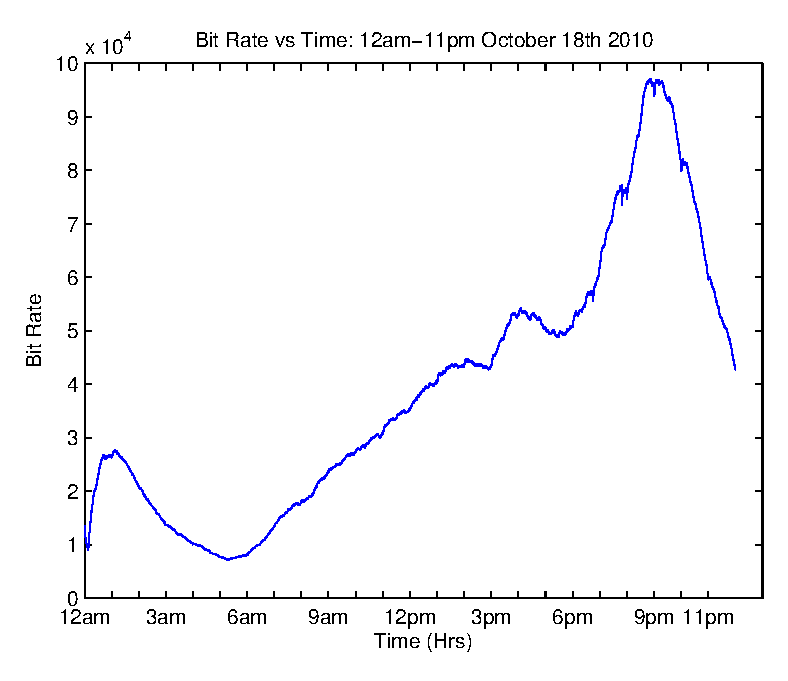
\includegraphics [width=4in]{final_project_NetMan_01.eps}

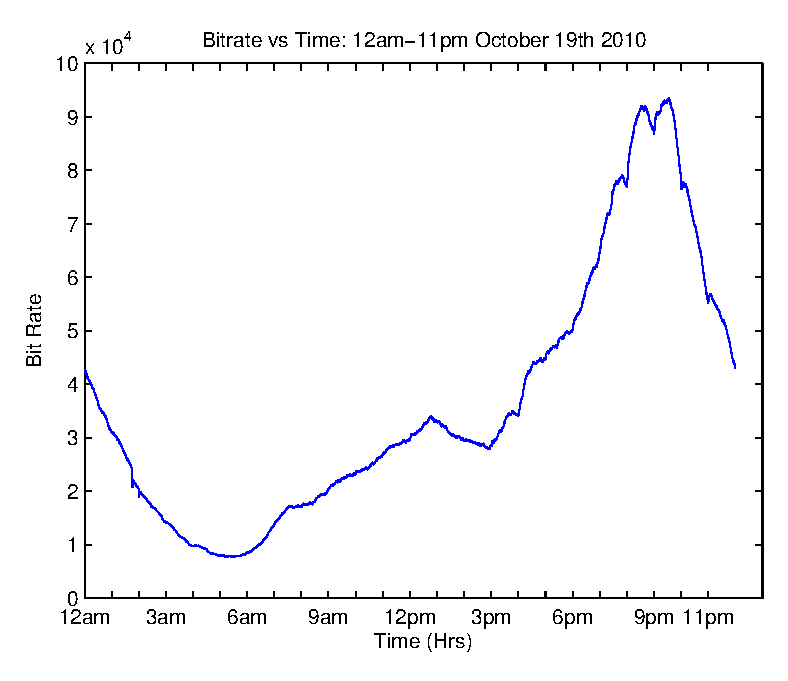
\includegraphics [width=4in]{final_project_NetMan_02.eps}

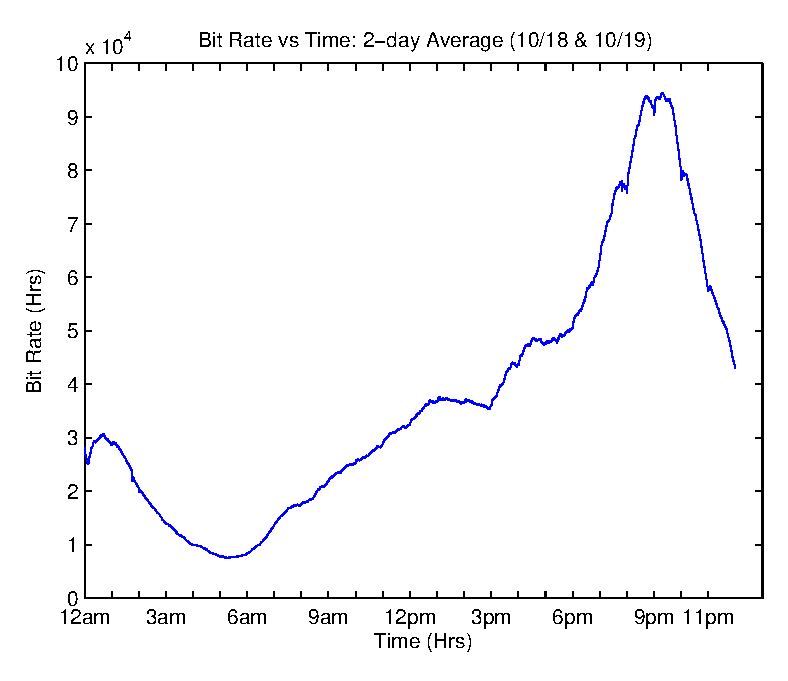
\includegraphics [width=4in]{final_project_NetMan_03.eps}

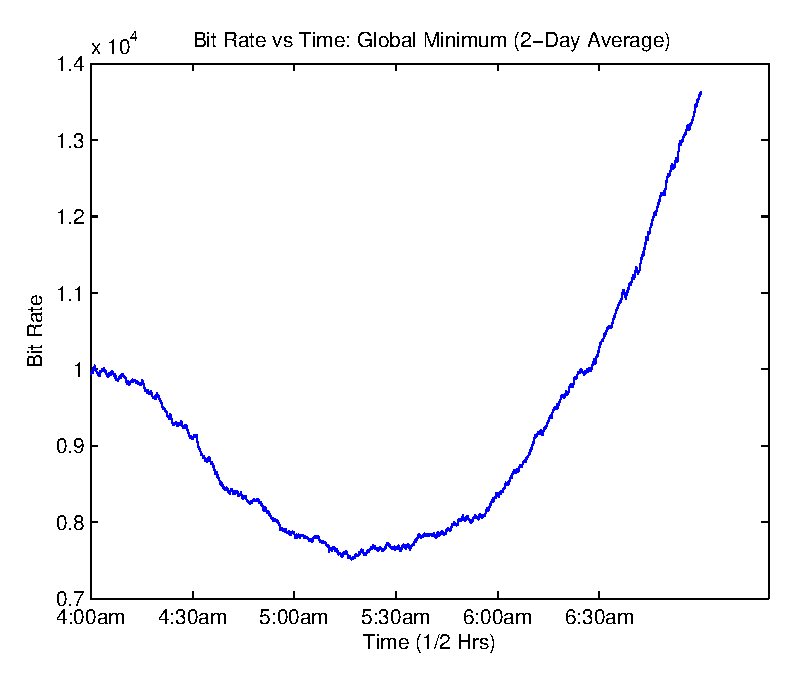
\includegraphics [width=4in]{final_project_NetMan_04.eps}

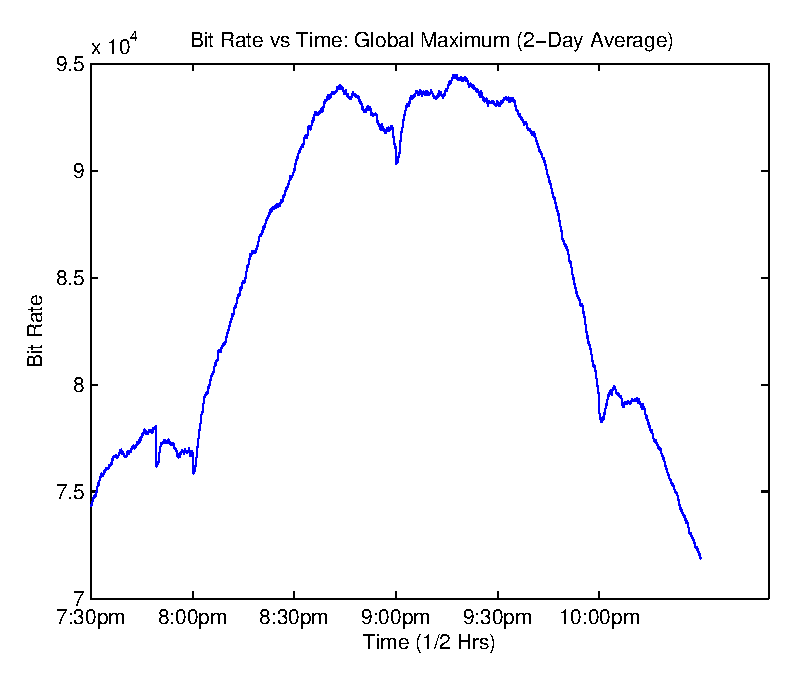
\includegraphics [width=4in]{final_project_NetMan_05.eps}


\subsection*{Part 4 - Provider Analysis}

\begin{verbatim}
%{
%Clear Unused Variables for use with aggregates
dat(:,6) = zeros(m,1);
dat(:,7) = zeros(m,1);

dat(1,7) = dat(1,8); %Initialize First Provider

k = 2;
no_match = 0;

for i = 1:m
   vsecs   = dat(i,2); % vewing seconds
   bitrate = dat(i,3);
   for j = 1:k % For each provider increment the corresponding slot
               % by the bitrate times the veiwing seconds
       if(dat(j,7) == dat(i,8))
           dat(j,6) = dat(j,6) + vsecs*bitrate;
       else if(j == k)
               no_match = 1;
           end
       end
   end

   if(no_match)
     k = k+1;
     dat(k,7) = dat(i,8);
     dat(k,6) = vsecs*bitrate;
     no_match = 0;
   end

end
%}
\end{verbatim}



\end{document}
    
